%------------------------------------------%
% Cannabis Data Science
% Date: 12/1/2021
%------------------------------------------%
\documentclass[xcolor={dvipsnames}]{beamer}
\hypersetup{pdfpagemode=FullScreen}
\mode<presentation>{
  \usetheme{Boadilla}
  \usecolortheme{orchid}
  \usefonttheme{default}
  \setbeamertemplate{navigation symbols}{}
  \setbeamertemplate{caption}[numbered]
} 
\usepackage[english]{babel}
\usepackage[utf8x]{inputenc}
\setbeamersize{text margin left=0.5in,text margin right=0.5in}

\usepackage[dvipsnames]{xcolor}
\definecolor{DarkGreen}{RGB}{2, 48, 32}
\definecolor{CalyxGreen}{RGB}{34, 153, 84}
\definecolor{DarkOrange}{RGB}{199, 0, 57}
\definecolor{LightOrange}{RGB}{255, 87, 51}
\definecolor{LightGreen}{RGB}{218, 247, 166}
\definecolor{LightYellow}{RGB}{255, 195, 0}

\setbeamercolor*{palette primary}{bg=LightGreen, fg = DarkGreen}
\setbeamercolor*{palette secondary}{bg=LightGreen, fg=DarkGreen}
\setbeamercolor*{palette tertiary}{bg=LightGreen, fg = DarkGreen}
%\setbeamercolor*{palette quaternary}{bg=myNewColorD, fg = green}

%------------------------------------------%
% Packages
%------------------------------------------%
\usepackage{amsmath}
\renewcommand*\footnoterule{} %No sperating line on footnote
\usepackage{mathtools} %ANNOTATING EQUATIONS
\usepackage{hhline} %DOUBLBARS
\usepackage[super]{nth}
\usepackage{graphicx, caption, subcaption}

%------------------------------------------%
% Commands
%------------------------------------------%
\newcommand\T{\rule{0pt}{2.5ex}} %TOPSTRUT
\newcommand\B{\rule[-1.25ex]{0pt}{0pt}} %BOTTOMSTRUT
\newenvironment<>{varblock}[2][.9\textwidth] %RESIZED BLOCKS
  {\setlength{\textwidth}{#1}
  \begin{actionenv}#3
    \def\insertblocktitle{#2}\par
    \usebeamertemplate{block begin}}
  {\par\usebeamertemplate{block end}
  \end{actionenv}}
\defbeamertemplate{enumerate item}{largeball} %LARGE BALLS
{\begin{pgfpicture}{-1ex}{-0.65ex}{1.5ex}{1.5ex}
\usebeamercolor[fg]{item projected}
{\pgftransformscale{2.5}\pgftext{\Large\pgfuseshading{bigsphere}}}
{\pgftransformshift{\pgfpoint{0pt}{0.5pt}}
\pgftext{\usebeamerfont*{item projected}\small\insertenumlabel}}
\end{pgfpicture}}
\usepackage{tikz} % FANCY ARROWS
\usepackage{xparse}
\NewDocumentCommand\UpArrow{O{2.0ex} O{black}}{%
   \mathrel{\tikz[baseline] \draw [->, line width=0.5pt, #2] (0,0) -- ++(0,#1);}} % FANCY UPARROW
\NewDocumentCommand\DownArrow{O{2.0ex} O{black}}{%
   \mathrel{\tikz[baseline] \draw [<-, line width=0.5pt, #2] (0,0) -- ++(0,#1);}} % FANCY DOWNARROW
%\vskip 1cm
\makeatletter
\newcommand{\LeftEqNo}{\let\veqno\@@leqno}%LEFT EQUATION #'s
\makeatother

%------------------------------------------%
% Title
%------------------------------------------%
\title[Meetup]{}
\author{Cannabis Data Science}
\institute[]{\Large Meetup}
\date{December \nth{1}, 2021}
\begin{document}
\begin{frame}{}
  
\includegraphics[scale=0.075]{images/logos/cannlytics_logo_with_text_light.png}
  \titlepage
\end{frame}

%------------------------------------------%
% Introduction
%------------------------------------------%

\section{Introduction}

\begin{frame}{}

{\large \textbf{Someone wiser than me once said...}}\vspace{0.5\baselineskip}\\


\textit{``The reason you study economics is so that you don't get fooled by economists.''}\vspace{1.5\baselineskip}\\

Original quote:\vspace{0.5\baselineskip}\\

\textit{``The purpose of studying economics is not to acquire a set of ready-made answers to economic questions, but to learn how to avoid being deceived by economists.''}\vspace{0.5\baselineskip}\\

- Joan Robinson, British Economist (1903 - 1983)

\end{frame}



% Massachusetts Licensee Types

\begin{frame}{}

{\large \textbf{Cannabis Licenses by Type in Massachusetts}}\vspace{0.5\baselineskip}\\

\begin{figure}
    \begin{subfigure}[t]{1\textwidth}
      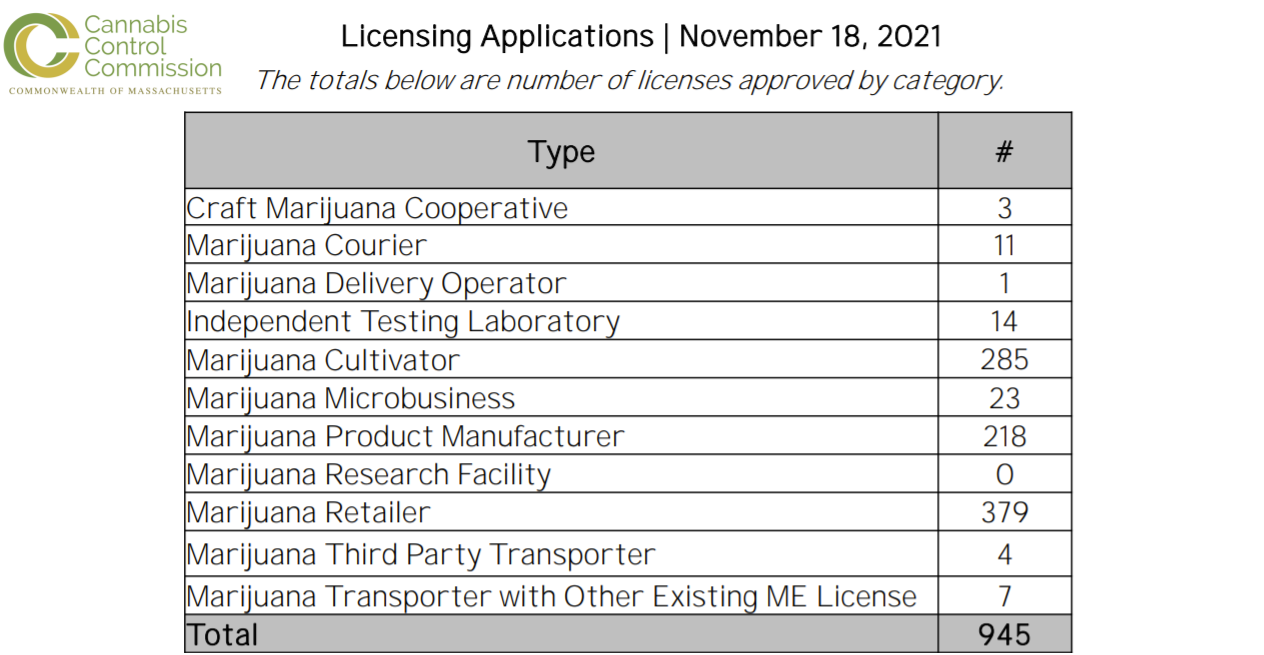
\includegraphics[width=\textwidth]{images/ma_applications_types.png}
    \end{subfigure}
    \caption*{\tiny Source: Massachusetts Cannabis Control Commission}
\end{figure}


\end{frame}

% Massachusetts Licensee Count

\begin{frame}{}

{\large \textbf{Cannabis Licenses Approval Stage in Massachusetts}}\vspace{0.5\baselineskip}\\

\begin{figure}
    \begin{subfigure}[t]{1\textwidth}
      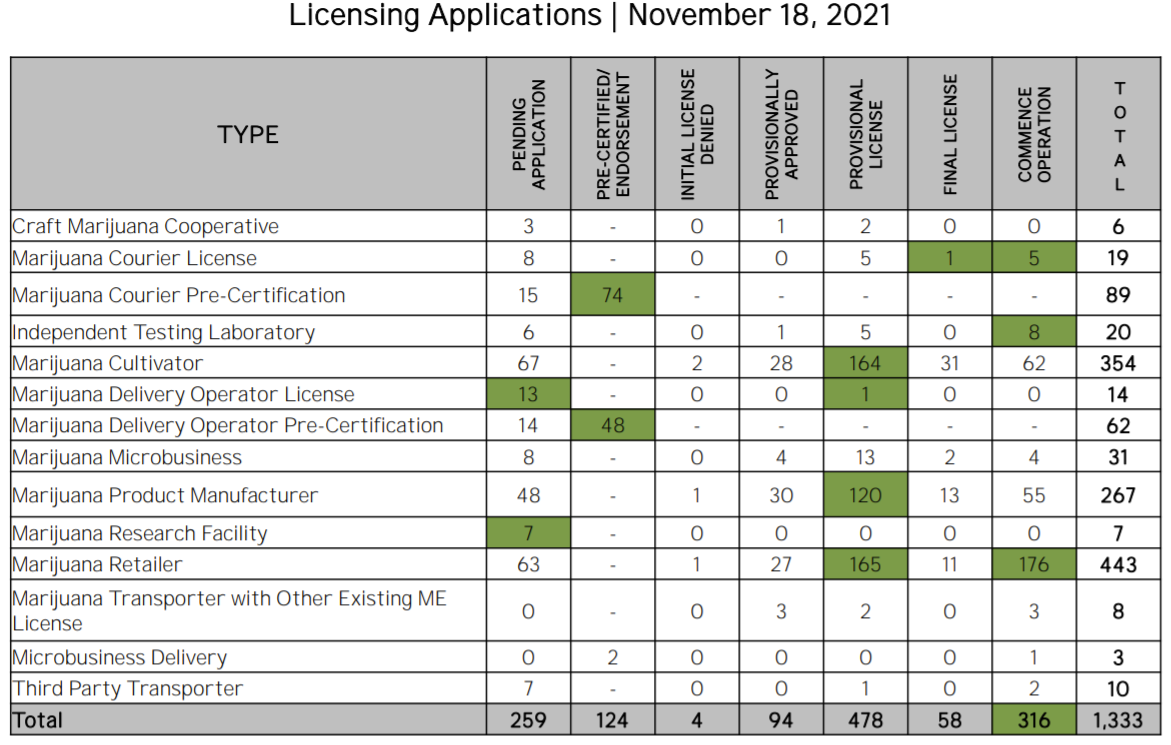
\includegraphics[width=\textwidth]{images/ma_licensees_stage_count.png}
    \end{subfigure}
    \caption*{\tiny Source: Massachusetts Cannabis Control Commission}
\end{figure}


\end{frame}


% Dispensary Statistics

\begin{frame}{}

{\large \textbf{Dispensary Statistics}}\vspace{0.5\baselineskip}\\

\begin{figure}
    \begin{subfigure}[t]{1\textwidth}
      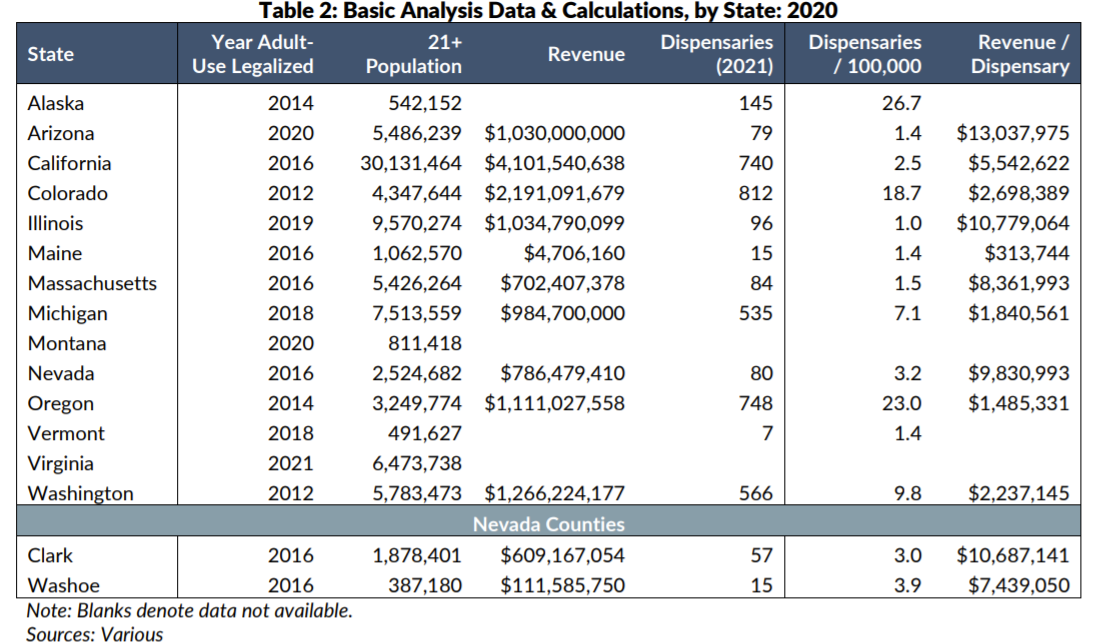
\includegraphics[width=\textwidth]{images/dispensary_statistics.png}
    \end{subfigure}
    \caption*{\tiny Source: Nevada Cannabis Dispensary Market Overview Technical Memorandum}
\end{figure}


\end{frame}

% Market Structure p{3cm}
\begin{frame}{}

{\large \textbf{Market Structure}}\vspace{0.5\baselineskip}\\

{\scriptsize
\begin{tabular}{ |l|l|l|l|  }
 \hline
 Market Structure	& Number of Firms & Barriers to Entry & Market Power\\
 \hline
Perfect Competition & $\infty$ & None & None\\
\hline
Monopolistic Competition & Many  & Low & Low\\
\hline
Oligopoly & Few & High & Medium\\
\hline
Monopoly & 1 & Blocked & High\\
 \hline
\end{tabular}
}

\end{frame}


% Research Question

\begin{frame}{}

{\large \textbf{Research Question}: What is the relationship between dispensaries per capita and revenue per dispensary?}\vspace{0.5\baselineskip}\\

\begin{figure}
    \begin{subfigure}[t]{1\textwidth}
      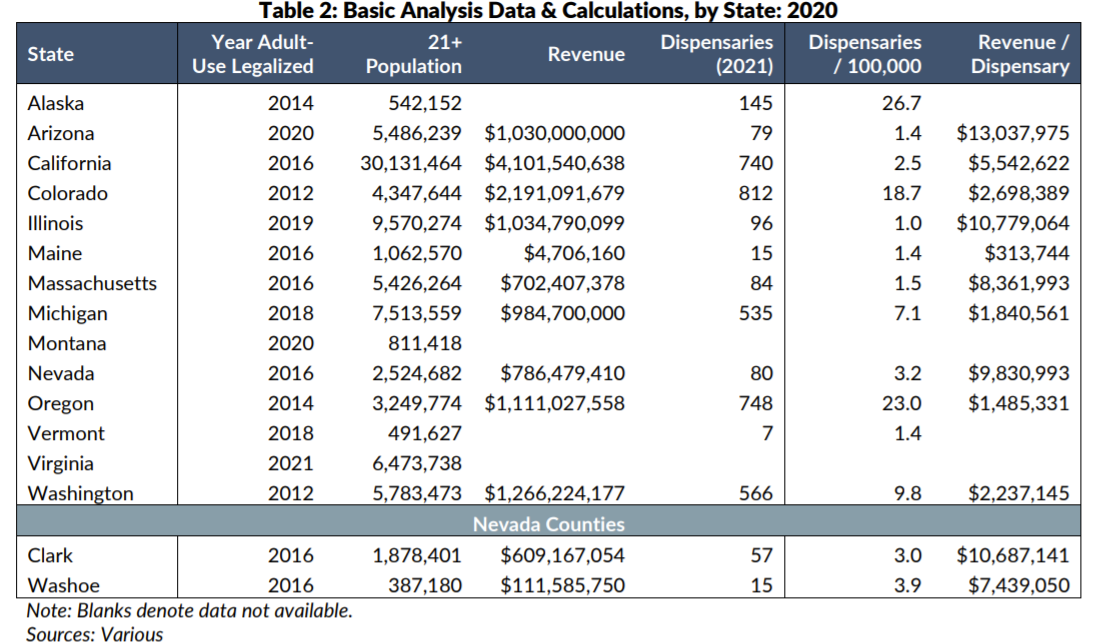
\includegraphics[width=\textwidth]{images/dispensary_statistics.png}
    \end{subfigure}
    \caption*{\tiny Source: Nevada Cannabis Dispensary Market Overview Technical Memorandum}
\end{figure}

\end{frame}


% Panel Data
\begin{frame}{}

{\large \textbf{Panel Data}}\vspace{0.5\baselineskip}\\

A panel has the form

\begin{figure}
    \begin{subfigure}[t]{.5\textwidth}
      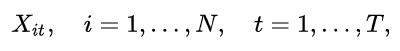
\includegraphics[width=\textwidth]{images/panel.png}
    \end{subfigure}
\end{figure}

where $i$ is the individual dimension and $t$ is the time dimension.\vspace{0.5\baselineskip}\\

A general panel data regression model is written as

\begin{figure}
    \begin{subfigure}[t]{.3\textwidth}
      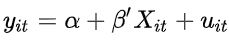
\includegraphics[width=\textwidth]{images/regression.png}
    \end{subfigure}
\end{figure}

where

\begin{figure}
    \begin{subfigure}[t]{.25\textwidth}
      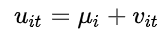
\includegraphics[width=\textwidth]{images/errors.png}
    \end{subfigure}
\end{figure}

Estimation with a \textbf{fixed effects} or \textbf{random effects} model depends on assumptions about $\mu_i$, the individual-specific, time-invariant effects.

\end{frame}



\section{Application}

%------------------------------------------%
% Takeaway
%------------------------------------------%

\begin{frame}{}

{\large \textbf{Future work}: Look at geographic distribution of licensees}\vspace{0.5\baselineskip}\\

\begin{figure}
    \begin{subfigure}[t]{1\textwidth}
      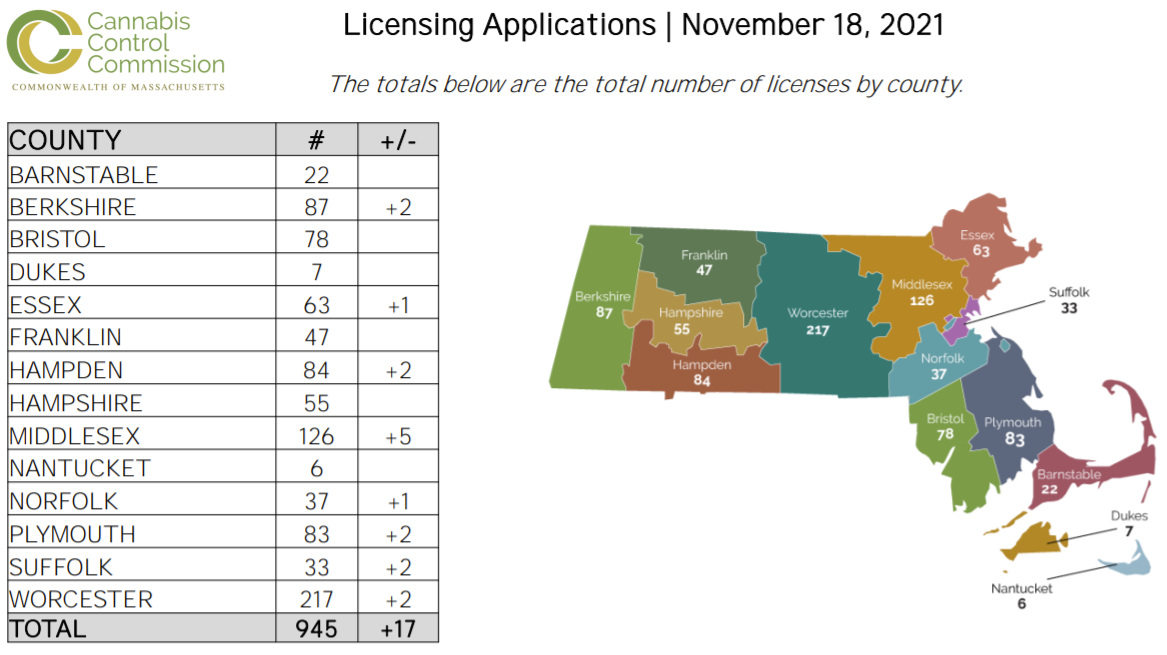
\includegraphics[width=\textwidth]{images/ma_application_map.png}
    \end{subfigure}
\end{figure}

\begin{center}
\begin{minipage}{3.85in}
Thank you for coming.
\end{minipage}
\end{center}

\end{frame}

%------------------------------------------%
\end{document}
%------------------------------------------%
